\begin{figure*}[t]   
    \vspace{3mm}
    \centering
    % \vspace{-0.5cm}
    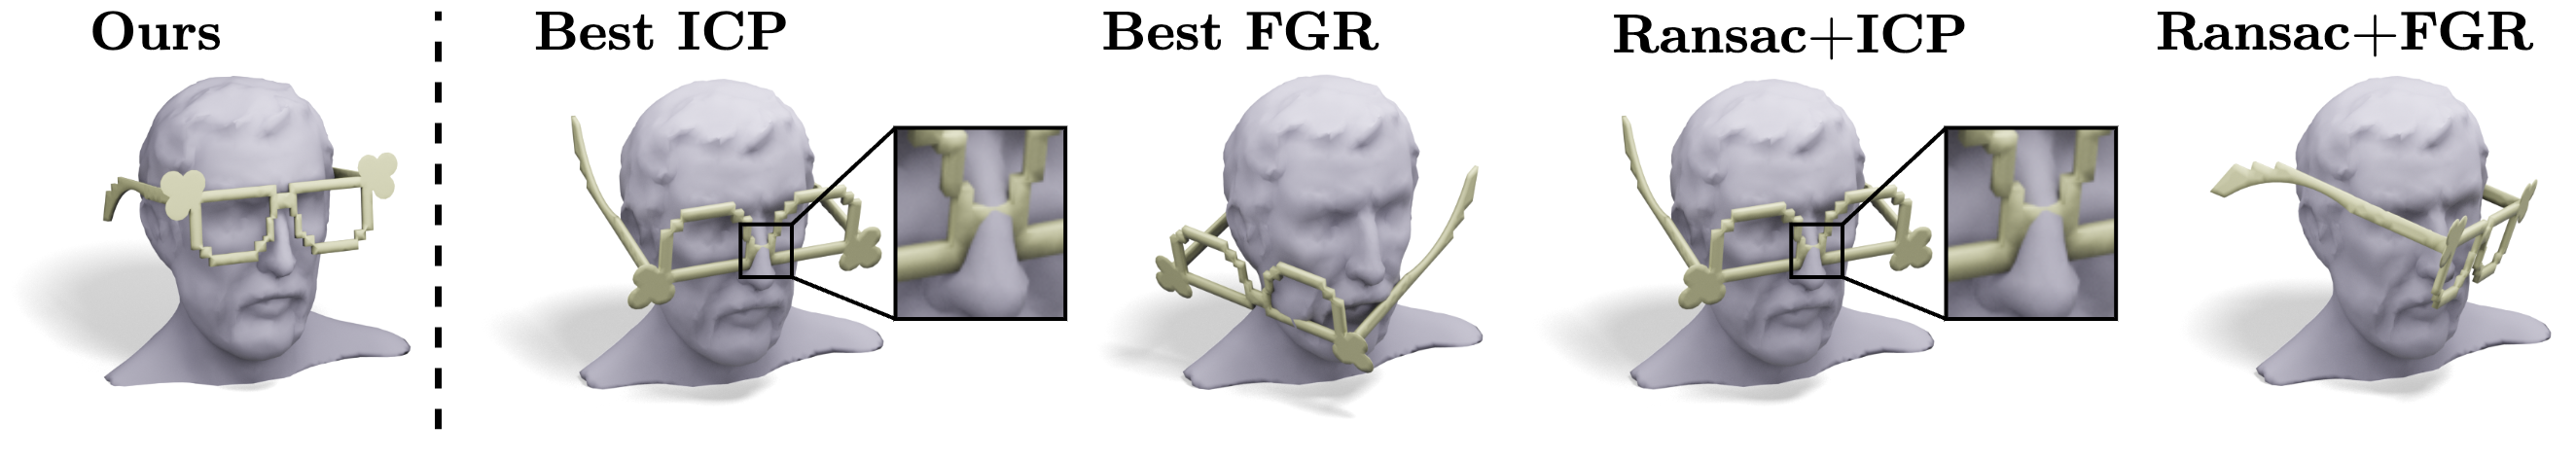
\includegraphics[width=\textwidth]{figures/comparison/comparison.png}
        \captionof{figure}{Unlike ours (left), classical registration algorithms like ICP contain no semantic guidance: therefore, they will produce unrealistic configurations; e.g., glasses that sit on the eyes upside down. These algorithms are also not designed to avoid intersections; therefore, they will produce many of them (see blowups). See supplementary materials for details of these methods.}
    %\vspace{-2cm}
    \label{fig:comparison}
\end{figure*}%
